\section{Results}

This section deals with the presentation and discussion of results.
The collected data are related to the obtained reward from the artificial neural network of the project.
With these data is possible to see what is the learning degree of the agent in the environment because the gained reward is intrinsically attached to the performance of the agent on the environment that it must go.
All the training environments were arranged by ROBOTIS, however, some alterations were done on the source code of the Gazebo simulation in order to use the simulated mobile robot and the reward function defined on this paper.

\subsection{Simulation Results}

A mobile robot with a SAC network was trained in order to make the experiments in the environments presented on Fig. \ref{fig:environments}, where the goal of the mobile robot is to get to the target.
The initial test used the first environment defined. It is shown in Fig. \ref{fig:frames_simenv1} a sequence of frames of the robot and the target. 
We can observe how the robot starts in an initial position distant from the target, navigating in order to reach the target.

\begin{figure}[htbp]
    \centering
    \begin{subfigure}[b]{0.115\textwidth}
        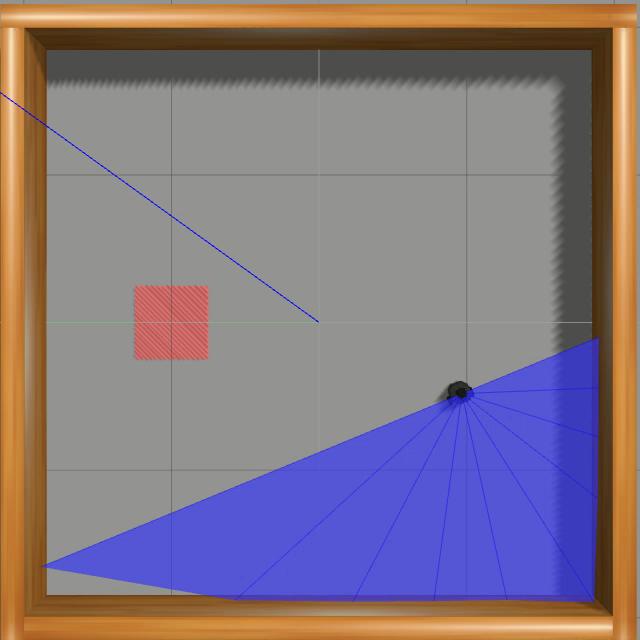
\includegraphics[width=\textwidth]{images/simenv1/1.png}
    \end{subfigure}
    \hfill
    \begin{subfigure}[b]{0.115\textwidth}
        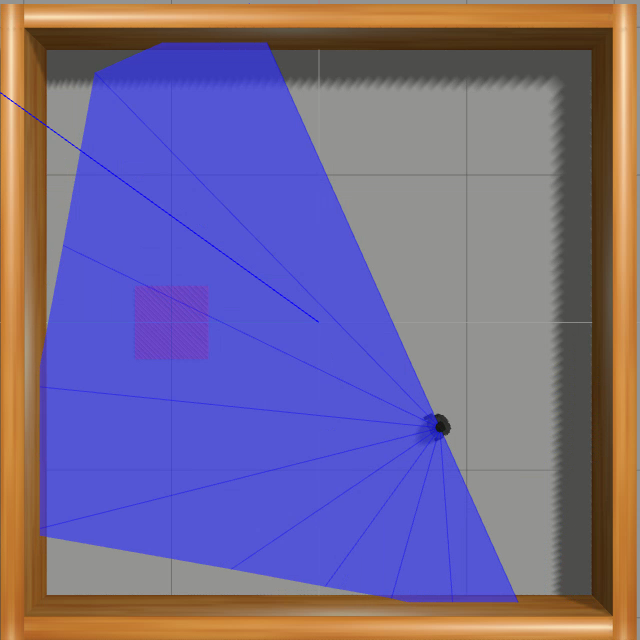
\includegraphics[width=\textwidth]{images/simenv1/2.png}
    \end{subfigure}
    \hfill
    \begin{subfigure}[b]{0.115\textwidth}
        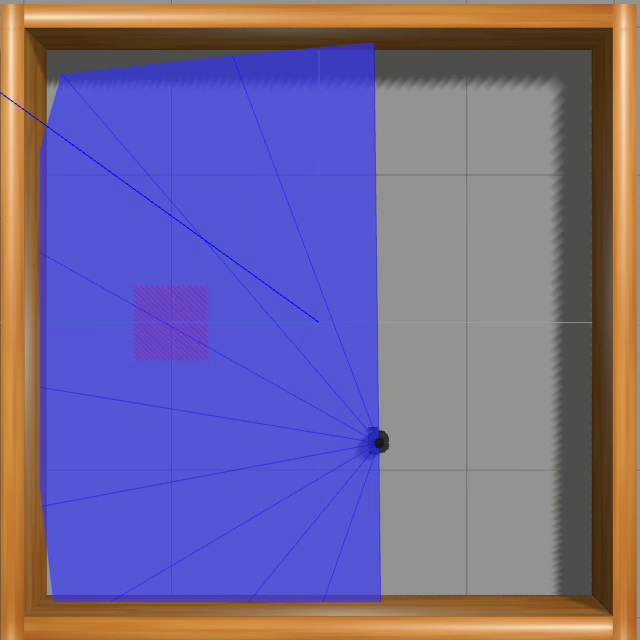
\includegraphics[width=\textwidth]{images/simenv1/3.png}
    \end{subfigure}
    \hfill
    \begin{subfigure}[b]{0.115\textwidth}
        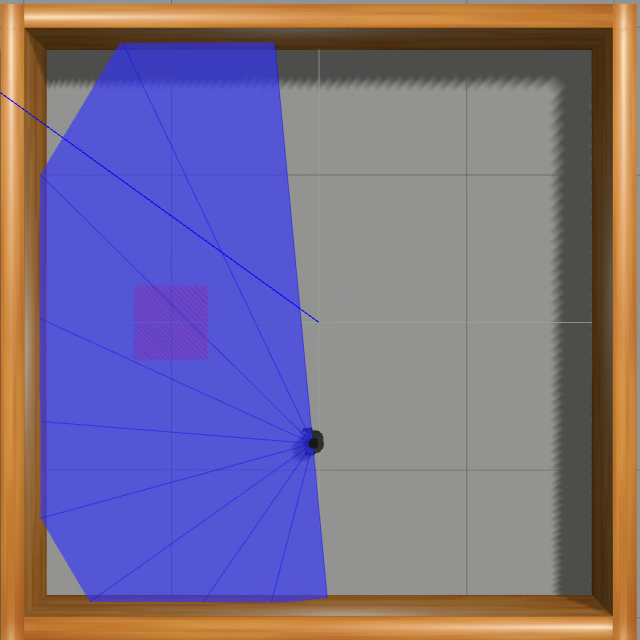
\includegraphics[width=\textwidth]{images/simenv1/4.png}
    \end{subfigure}
    \newline
    \begin{subfigure}[b]{0.115\textwidth}
        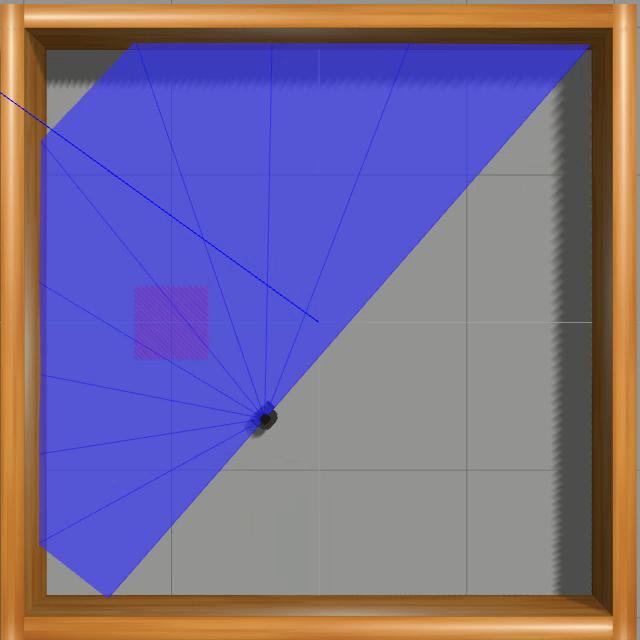
\includegraphics[width=\textwidth]{images/simenv1/5.png}
    \end{subfigure}
    \hfill
    \begin{subfigure}[b]{0.115\textwidth}
        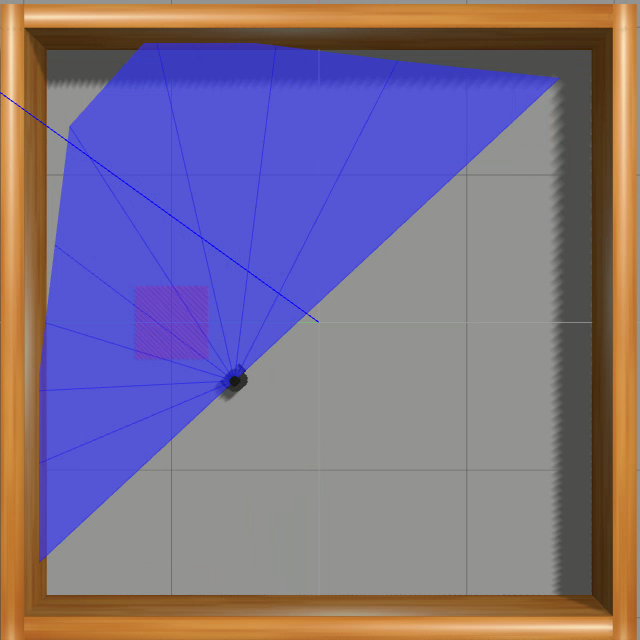
\includegraphics[width=\textwidth]{images/simenv1/6.png}
    \end{subfigure}
    \hfill
    \begin{subfigure}[b]{0.115\textwidth}
        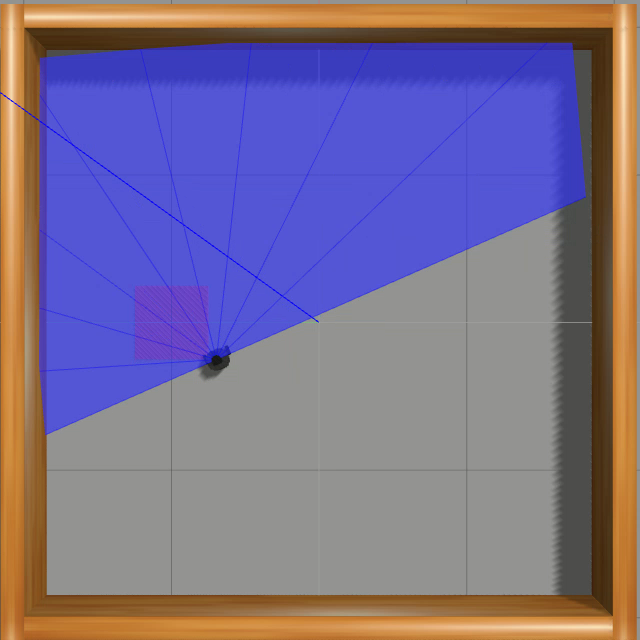
\includegraphics[width=\textwidth]{images/simenv1/7.png}
    \end{subfigure}
    \hfill
    \begin{subfigure}[b]{0.115\textwidth}
        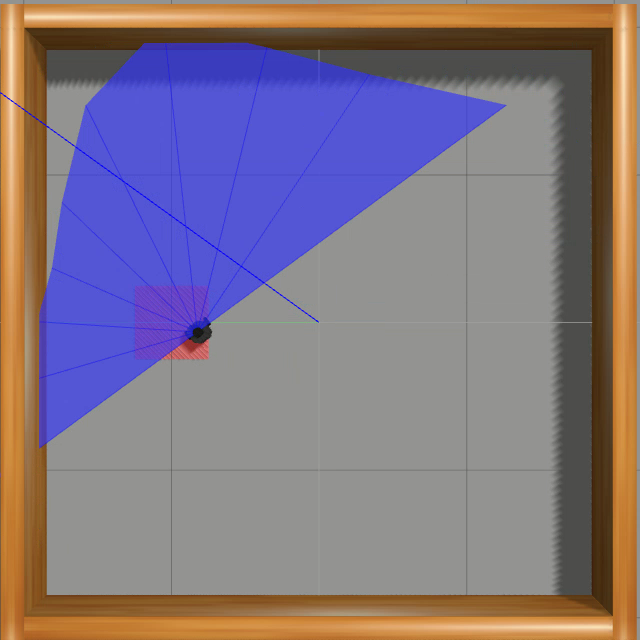
\includegraphics[width=\textwidth]{images/simenv1/8.png}
    \end{subfigure}
    \caption{Images sequence in the first simulated environment of the experiment.}\label{fig:frames_simenv1}
\end{figure}


The training results of the reward function of the first environment are shown in Fig. \ref{fig:stage_1}.
On the first episodes can be noticed a negative reward, this happens because the algorithm started and it was still learning.
This reward by episode means that the robot is trying to maximize the reward to complete the task.

\begin{figure}[htbp]
\centerline{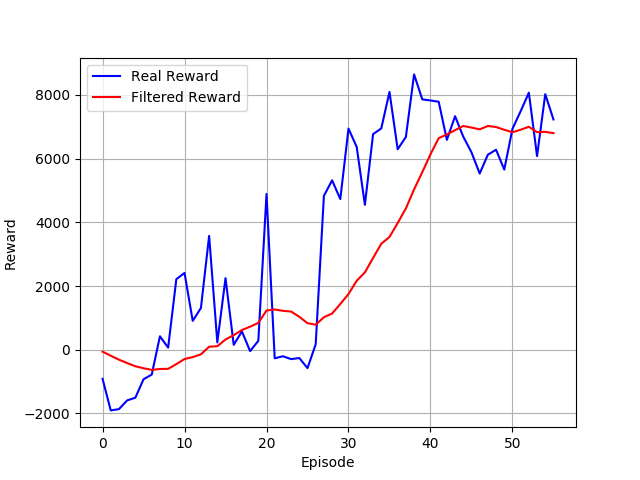
\includegraphics[width=\columnwidth]{images/stage_1.png}}
\caption{Rewards of the first environment.}
\label{fig:stage_1}
\end{figure}

In Fig. \ref{fig:stage_1} the $x$ axis represents the past episodes on the simulation, an episode is defined when the mobile robot arrives to the target in the map or collides with some obstacle. 
The $y$ axis in Fig. \ref{fig:stage_1} represents the total value of the reward that the robot received on the episode.
The reward, with the blue color, has a great variance, it was decided to use a moving average filter for better visualization of the results.

After the mobile robot has been trained on the first environment, the experiment was done in the second environment.
It is shown in Fig. \ref{fig:frames_simenv2} a sequence of the actions made by the Turtlebot from an initial position until it could arrive to the target after the training episodes.

\begin{figure}[htbp]
    \centering
    \begin{subfigure}[b]{0.115\textwidth}
        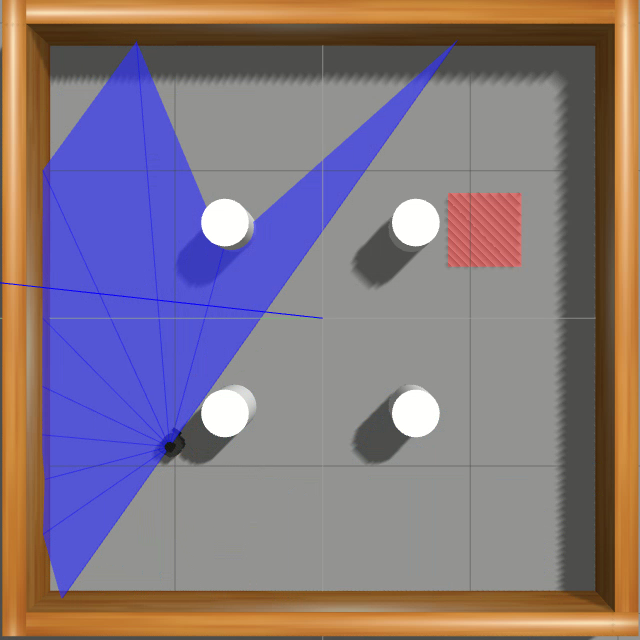
\includegraphics[width=\textwidth]{images/simenv2/1.png}
    \end{subfigure}
    \hfill
    \begin{subfigure}[b]{0.115\textwidth}
        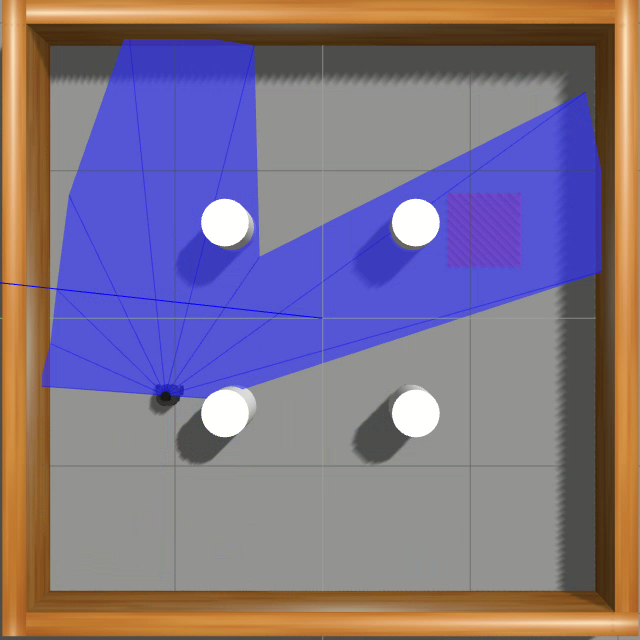
\includegraphics[width=\textwidth]{images/simenv2/2.png}
    \end{subfigure}
    \hfill
    \begin{subfigure}[b]{0.115\textwidth}
        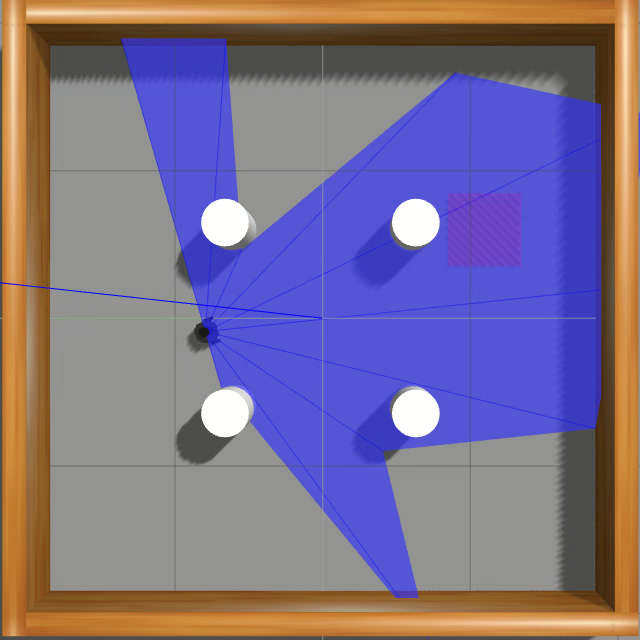
\includegraphics[width=\textwidth]{images/simenv2/3.png}
    \end{subfigure}
    \hfill
    \begin{subfigure}[b]{0.115\textwidth}
        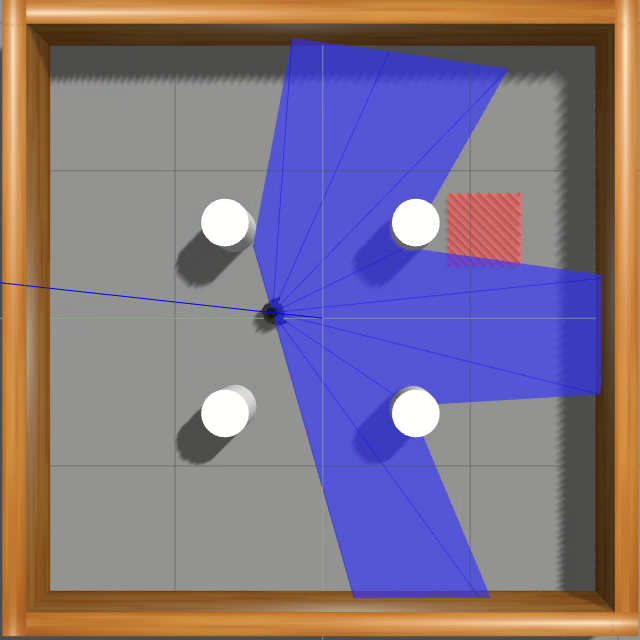
\includegraphics[width=\textwidth]{images/simenv2/4.png}
    \end{subfigure}
    \newline
    \begin{subfigure}[b]{0.115\textwidth}
        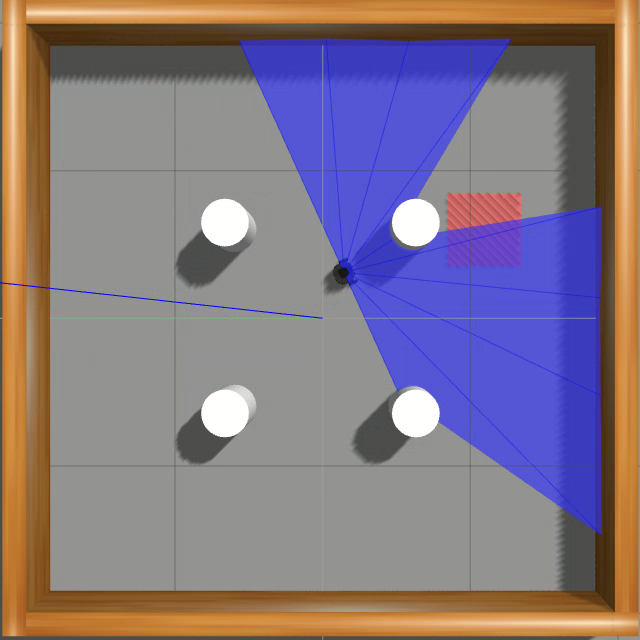
\includegraphics[width=\textwidth]{images/simenv2/5.png}
    \end{subfigure}
    \hfill
    \begin{subfigure}[b]{0.115\textwidth}
        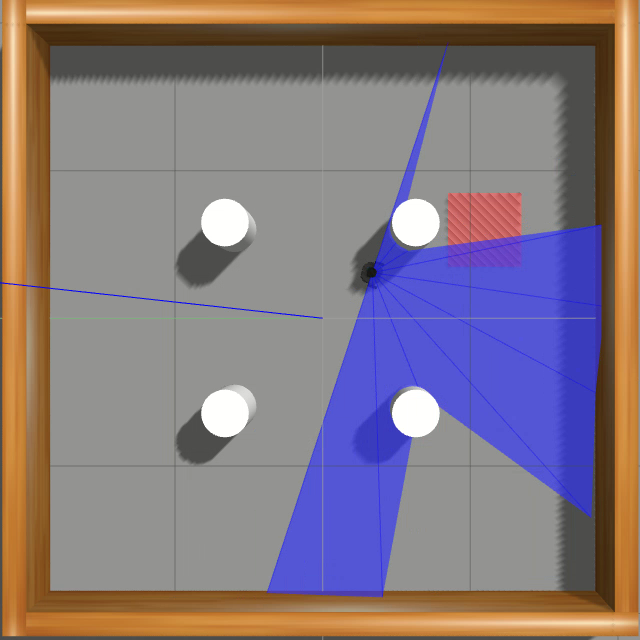
\includegraphics[width=\textwidth]{images/simenv2/6.png}
    \end{subfigure}
    \hfill
    \begin{subfigure}[b]{0.115\textwidth}
        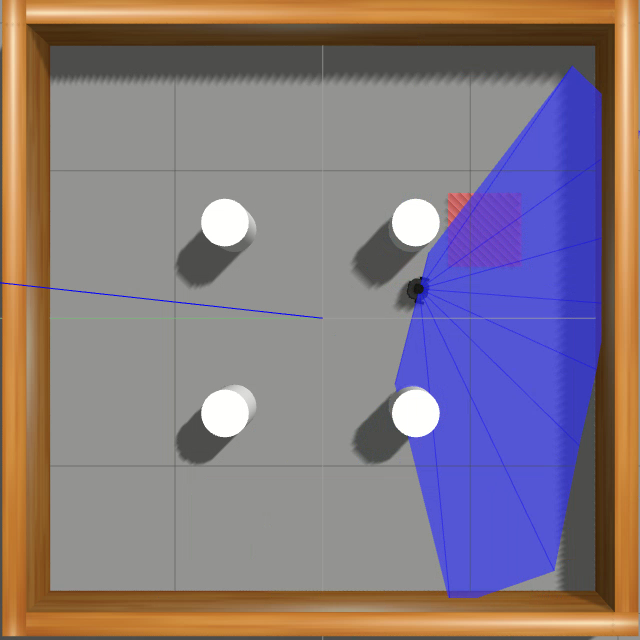
\includegraphics[width=\textwidth]{images/simenv2/7.png}
    \end{subfigure}
    \hfill
    \begin{subfigure}[b]{0.115\textwidth}
        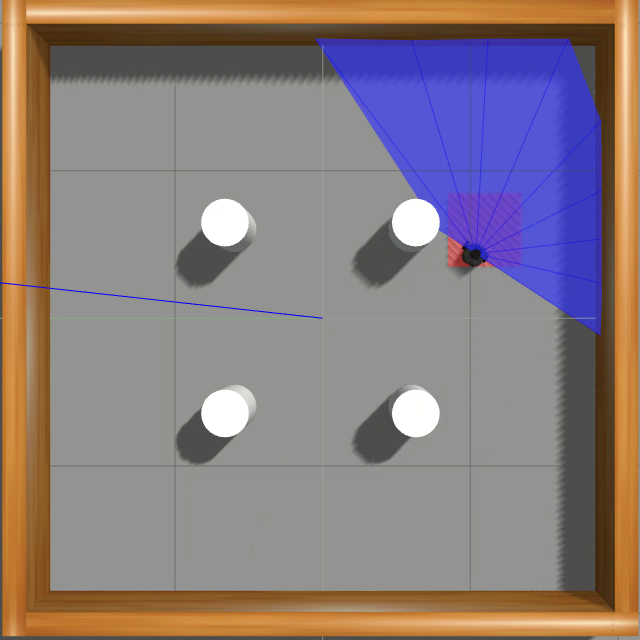
\includegraphics[width=\textwidth]{images/simenv2/8.png}
    \end{subfigure}
    \caption{Images sequence in the second simulated environment of the experiment.}\label{fig:frames_simenv2}
\end{figure}

The reward function results of the training process for the second environment are shown in Fig. \ref{fig:stage_2}.
Comparing this results with the last environment, we can observe that it needed more episodes so the robot could present good results.
It is noticed that with a more complex environment, exists the possibility that an agent could take a longer time to get a good performance.

\begin{figure}[htbp]
\centerline{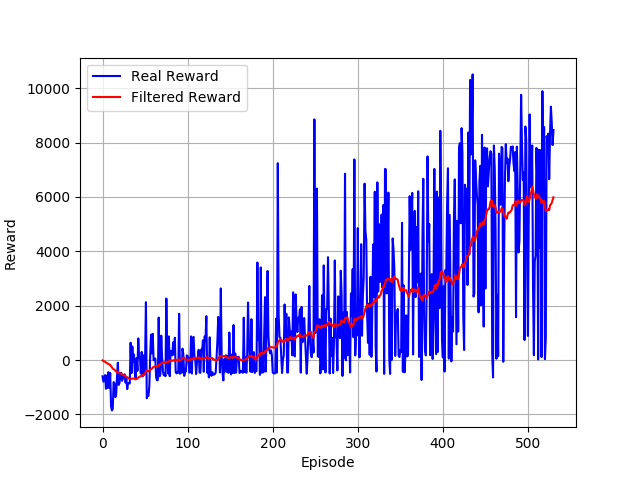
\includegraphics[width=\columnwidth]{images/stage_2.png}}
\caption{Rewards of the second environment.}
\label{fig:stage_2}
\end{figure}

\subsection{Experiments with Turtlebot}

After the training and validation of each simulation environment, there were used the two real environments, presented in the Fig. \ref{fig:real_environments}, for the testing of the SAC network in the real world.
With the target defined on the first real environment, it was executed the SAC network on the Turtlebot3.
In the graph, shown in Fig. \ref{fig:env1_graph}, is possible to see the trajectory made by the network to arrive to the target.
The robot starts at the point $(0, 0)$ and makes a trajectory to get to the target.
Fig. \ref{fig:frames_env1} shows by frames the trajectory made by the robot to complete the task.

\begin{figure}[htbp]
\centerline{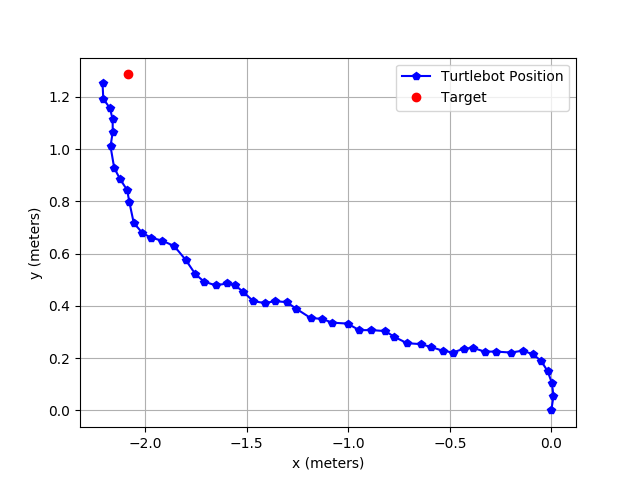
\includegraphics[width=\columnwidth]{images/test_env1.png}}
\caption{Trajectory of the Turtlebot3 in the first real environment}
\label{fig:env1_graph}
\end{figure}

\begin{figure}[htbp]
    \centering
    \begin{subfigure}[b]{0.115\textwidth}
        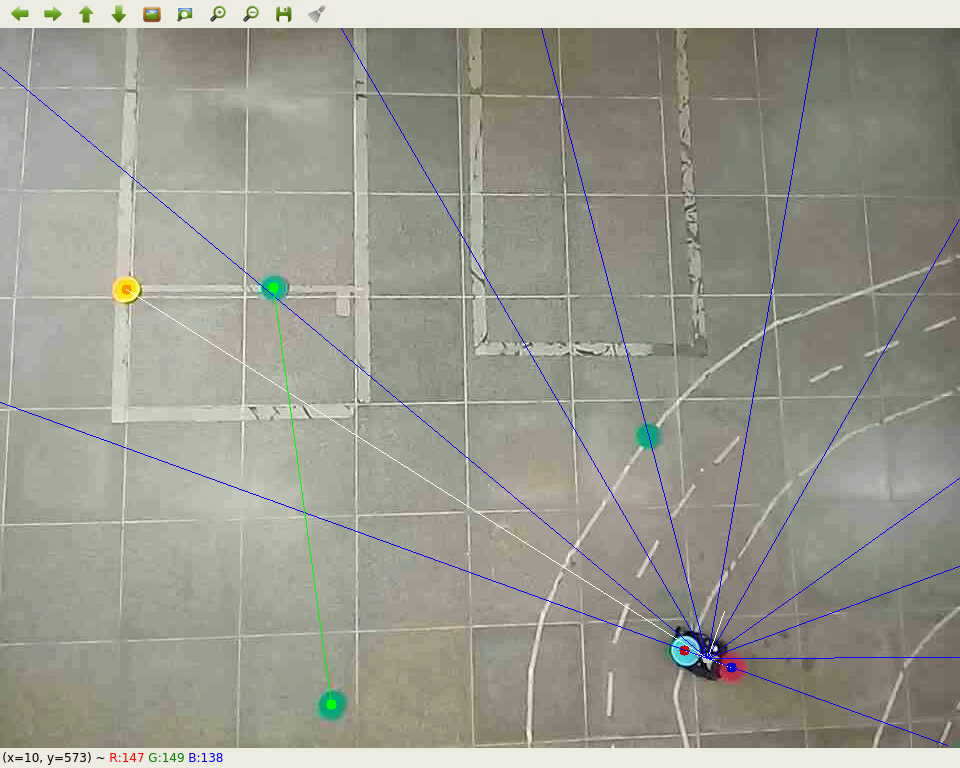
\includegraphics[width=\textwidth]{images/test_env1/1.png}
    \end{subfigure}
    \hfill
    \begin{subfigure}[b]{0.115\textwidth}
        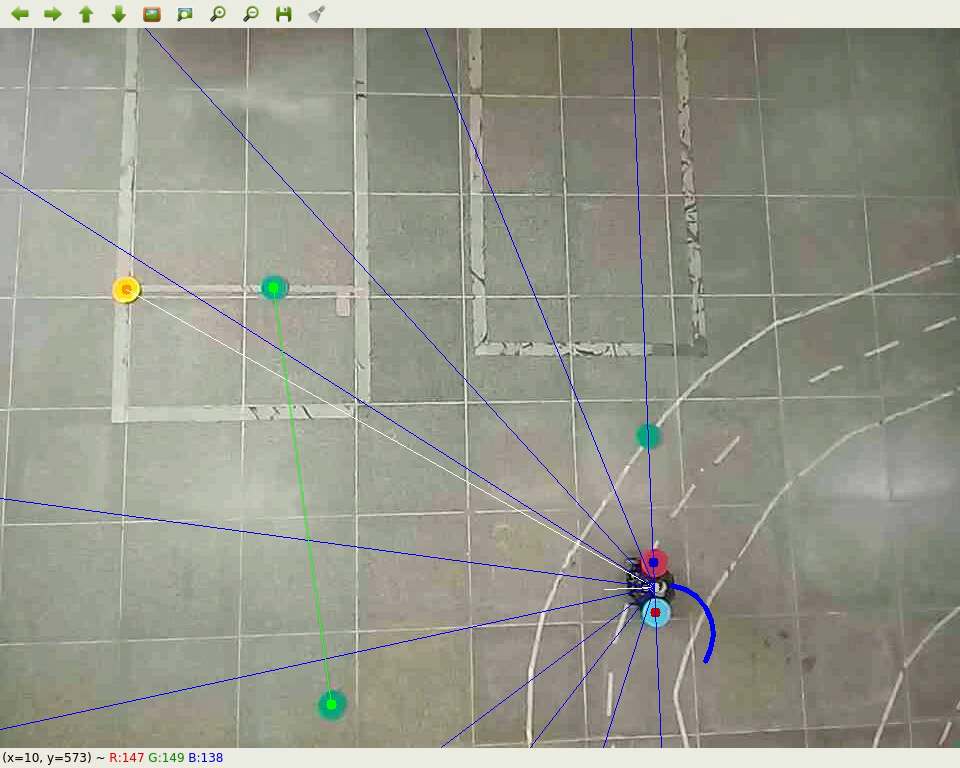
\includegraphics[width=\textwidth]{images/test_env1/2.png}
    \end{subfigure}
    \hfill
    \begin{subfigure}[b]{0.115\textwidth}
        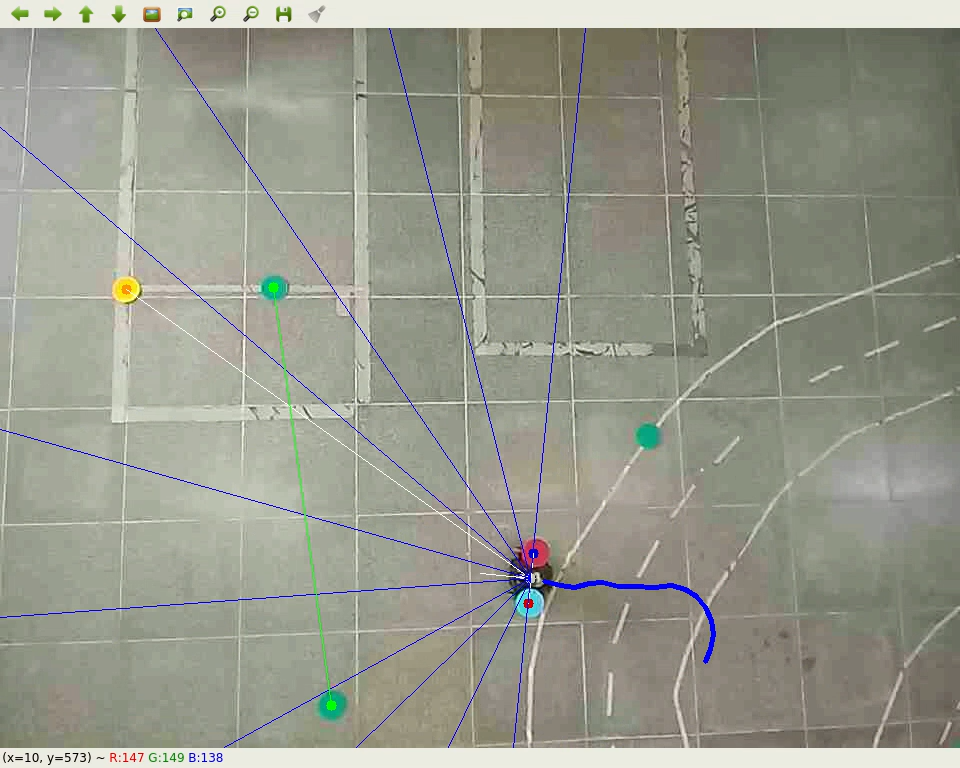
\includegraphics[width=\textwidth]{images/test_env1/3.png}
    \end{subfigure}
    \hfill
    \begin{subfigure}[b]{0.115\textwidth}
        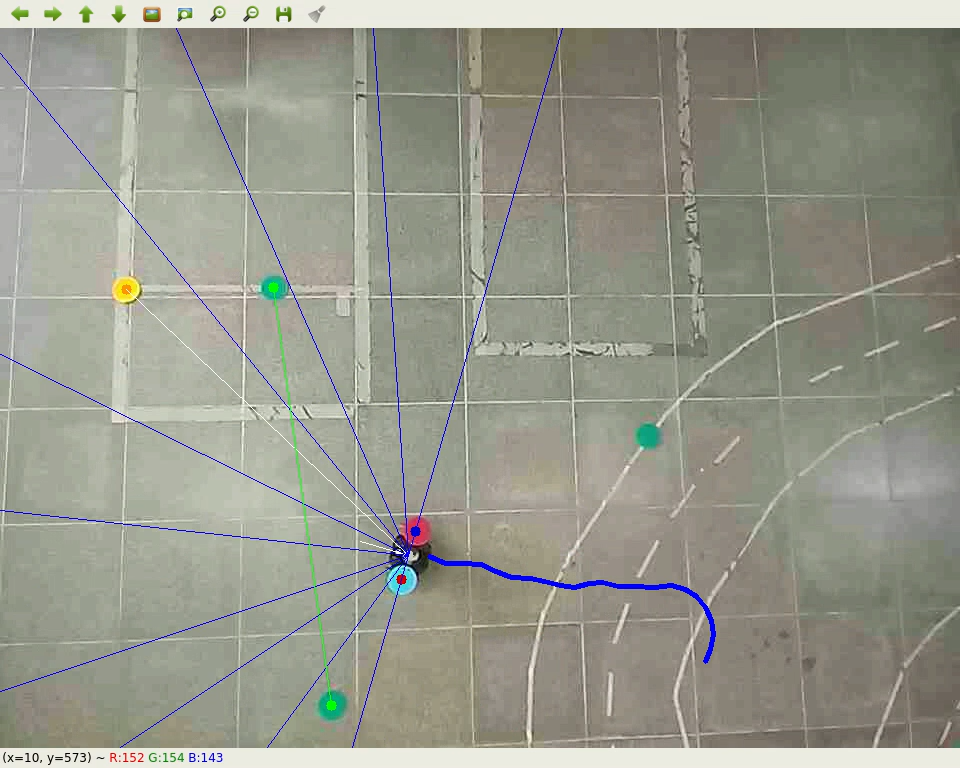
\includegraphics[width=\textwidth]{images/test_env1/4.png}
    \end{subfigure}
    \newline
    \begin{subfigure}[b]{0.115\textwidth}
        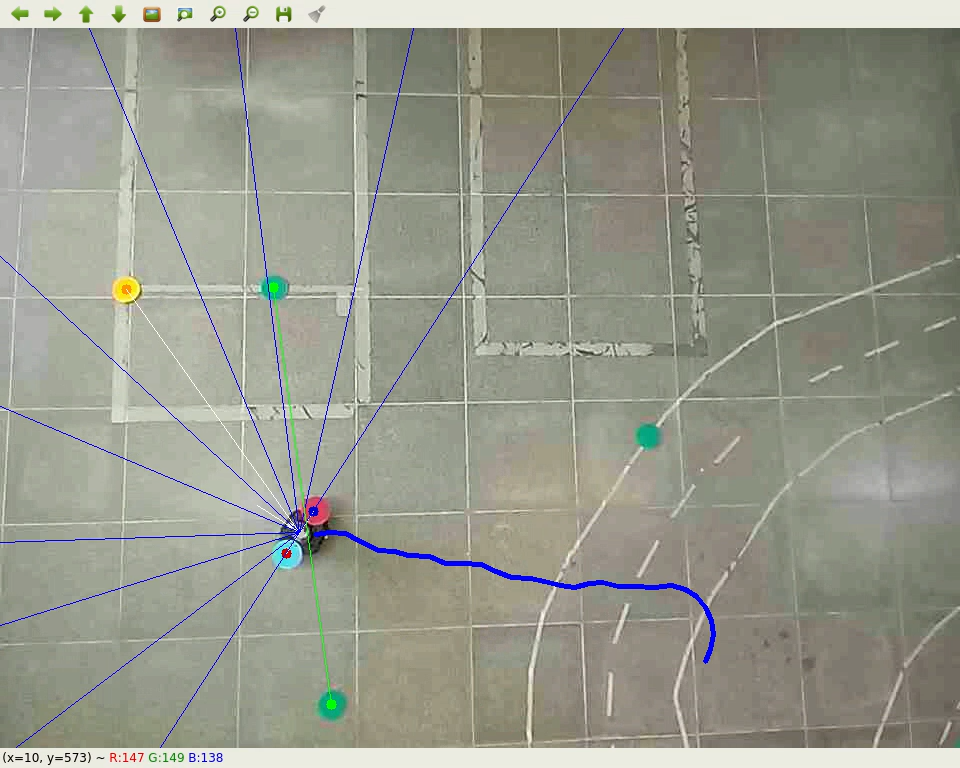
\includegraphics[width=\textwidth]{images/test_env1/5.png}
    \end{subfigure}
    \hfill
    \begin{subfigure}[b]{0.115\textwidth}
        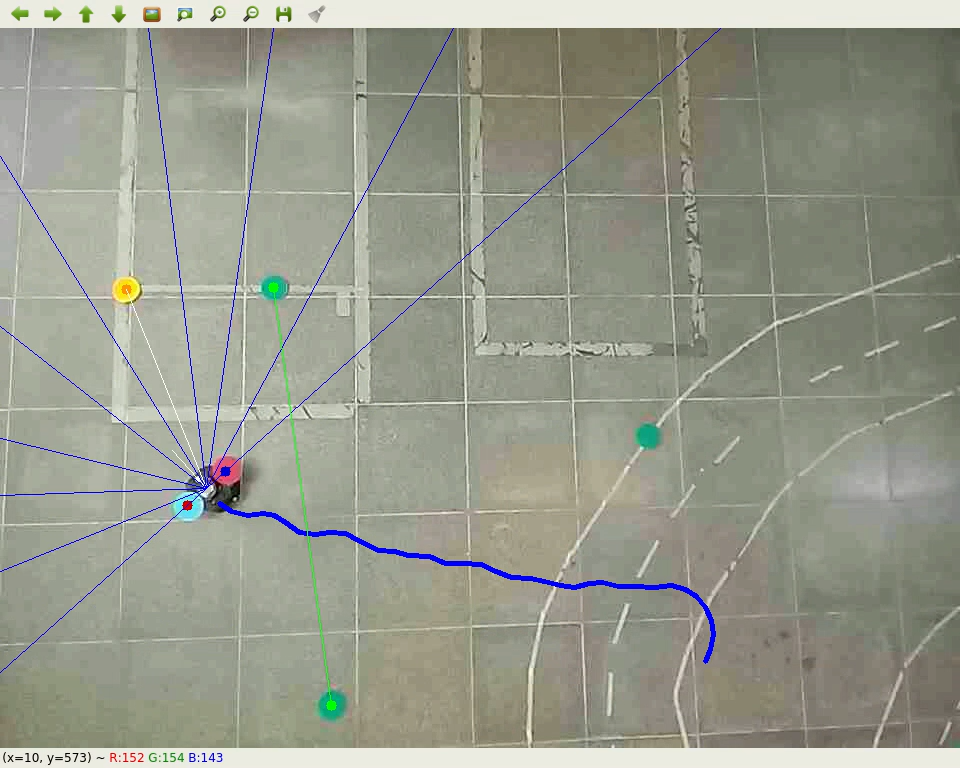
\includegraphics[width=\textwidth]{images/test_env1/6.png}
    \end{subfigure}
    \hfill
    \begin{subfigure}[b]{0.115\textwidth}
        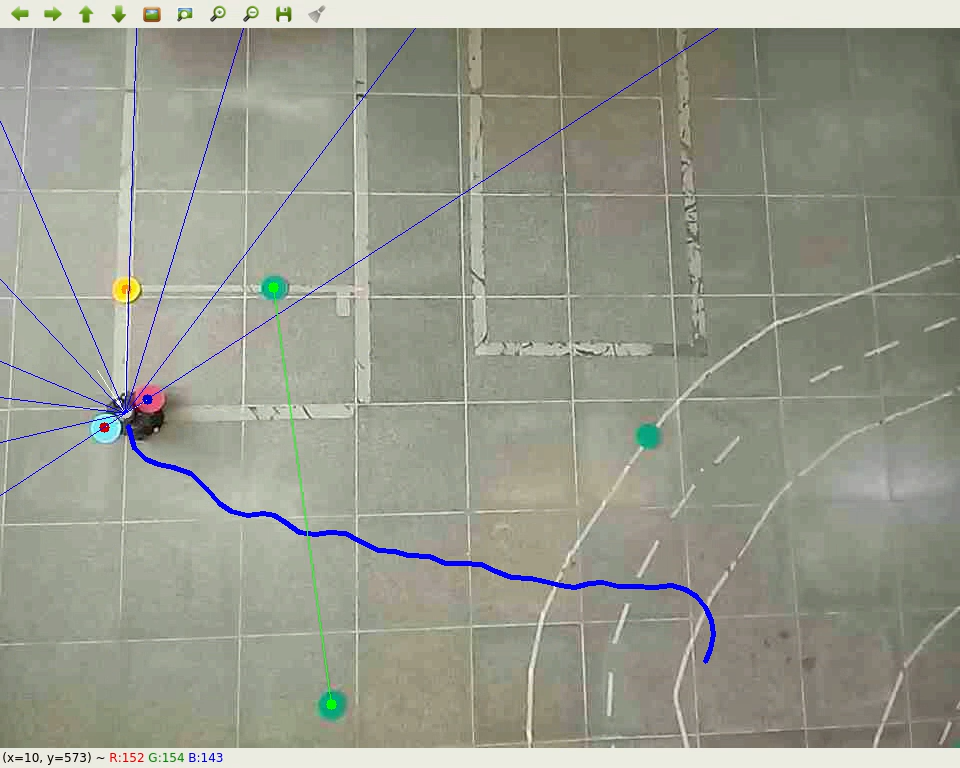
\includegraphics[width=\textwidth]{images/test_env1/7.png}
    \end{subfigure}
    \hfill
    \begin{subfigure}[b]{0.115\textwidth}
        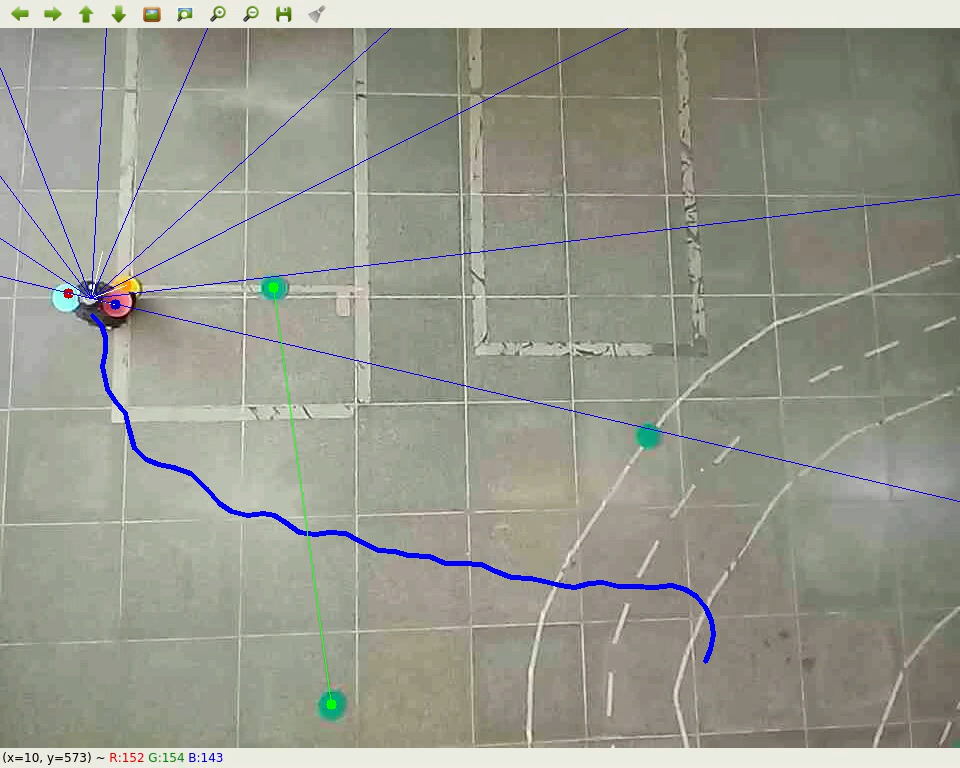
\includegraphics[width=\textwidth]{images/test_env1/8.png}
    \end{subfigure}
    \caption{Images sequence of the experiment on the Turtlebot3 in the first real environment.}\label{fig:frames_env1}
\end{figure}

For the final test of the network, it was used the second real environment.
In the graph, shown in Fig. \ref{fig:env2_graph}, the robot starts at the point $(0, 0)$ and even with obstacle the network was capable to arrive to the target. In Fig. \ref{fig:frames_env2} is shown by frames the trajectory made by the robot to complete the task. %So, with these results applied on real world environment we can see how effective can be a DDPG network trained in simulation environment
The robot was able to accomplish both tasks given in the real world environments.
This shows how effective can be the SAC networks, trained in a simulation environment, in completing complex tasks on physical environment.

\begin{figure}[htbp]
\centerline{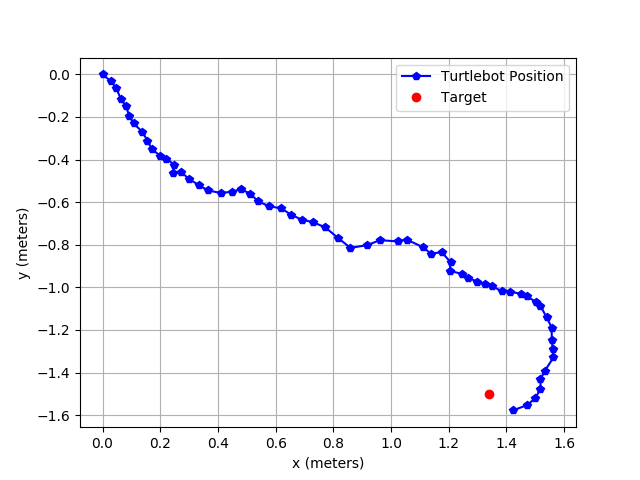
\includegraphics[width=\columnwidth]{images/test_env2.png}}
\caption{Trajectory of the Turtlebot3 in the second real environment}
\label{fig:env2_graph}
\end{figure}

\begin{figure}[htbp]
    \centering
    \begin{subfigure}[b]{0.115\textwidth}
        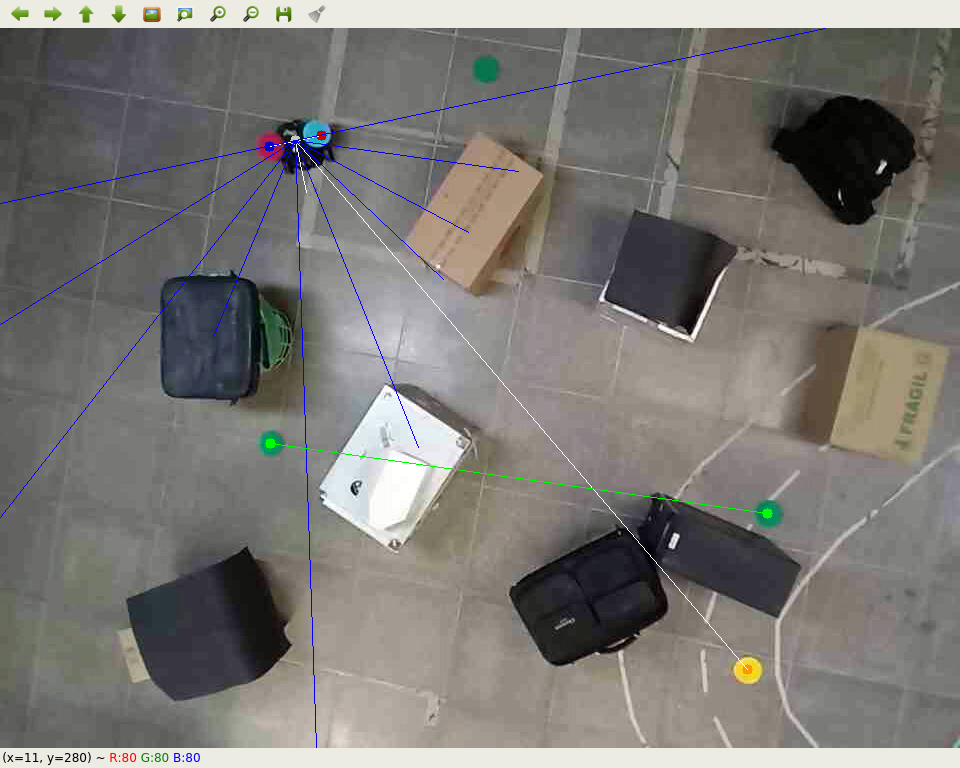
\includegraphics[width=\textwidth]{images/test_env2/1.png}
    \end{subfigure}
    \hfill
    \begin{subfigure}[b]{0.115\textwidth}
        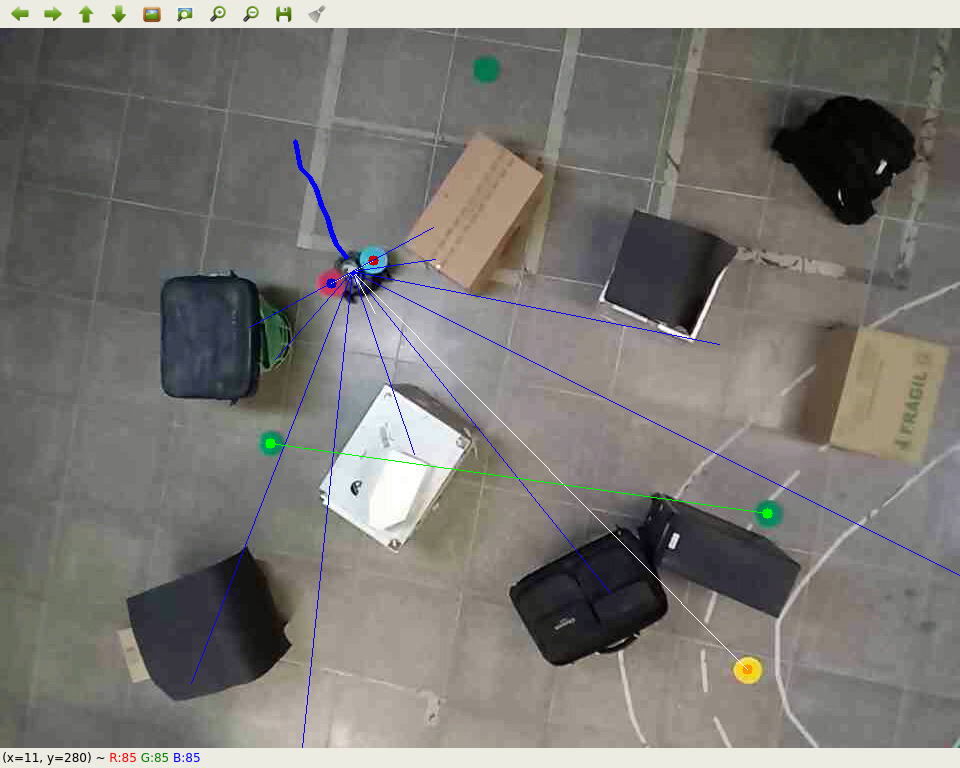
\includegraphics[width=\textwidth]{images/test_env2/2.png}
    \end{subfigure}
    \hfill
    \begin{subfigure}[b]{0.115\textwidth}
        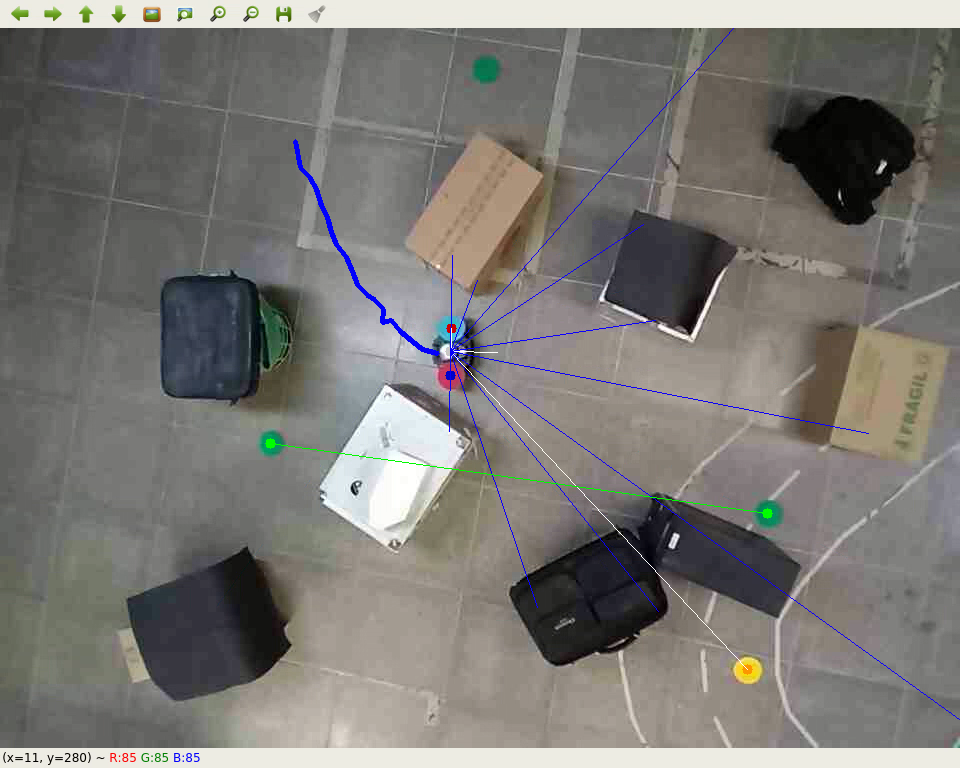
\includegraphics[width=\textwidth]{images/test_env2/3.png}
    \end{subfigure}
    \hfill
    \begin{subfigure}[b]{0.115\textwidth}
        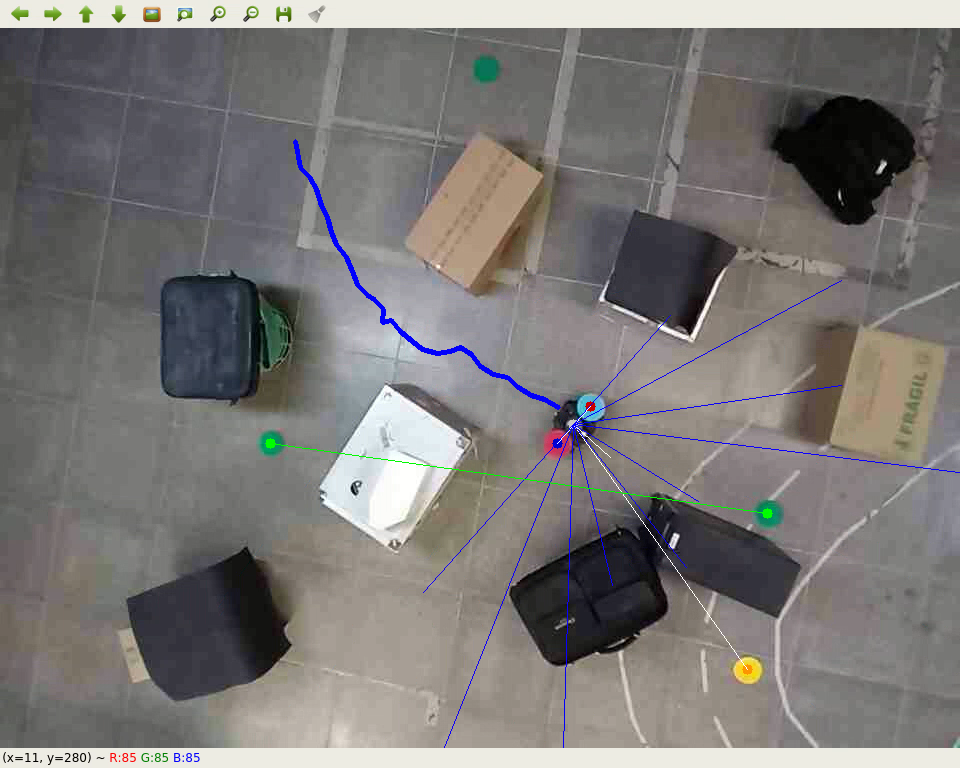
\includegraphics[width=\textwidth]{images/test_env2/4.png}
    \end{subfigure}
    \newline
    \begin{subfigure}[b]{0.115\textwidth}
        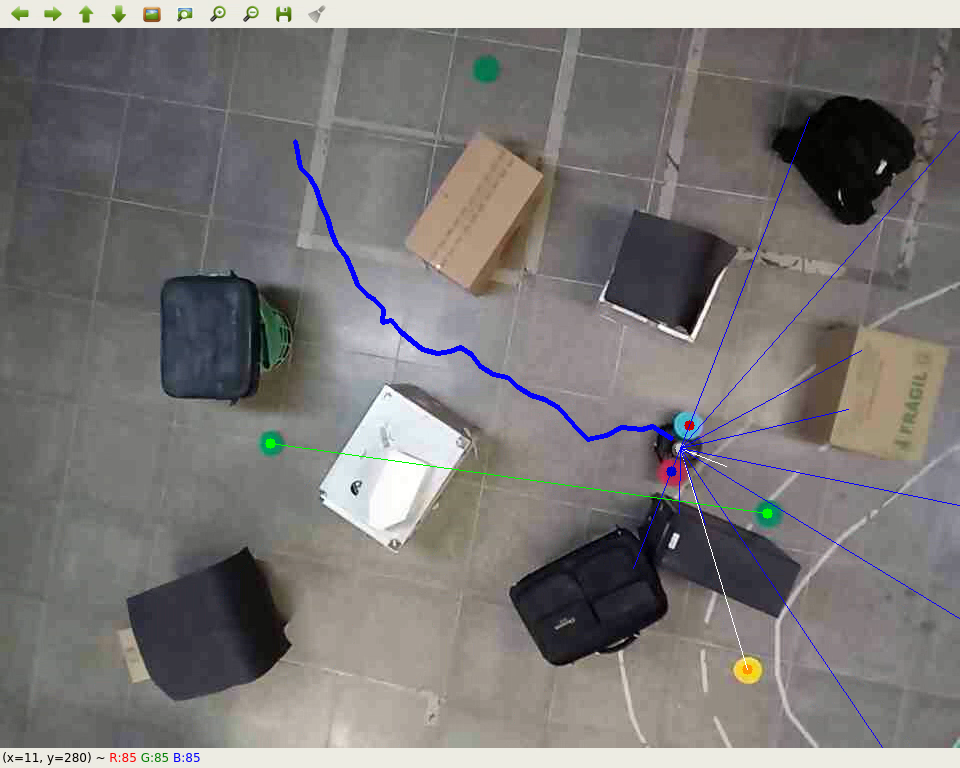
\includegraphics[width=\textwidth]{images/test_env2/5.png}
    \end{subfigure}
    \hfill
    \begin{subfigure}[b]{0.115\textwidth}
        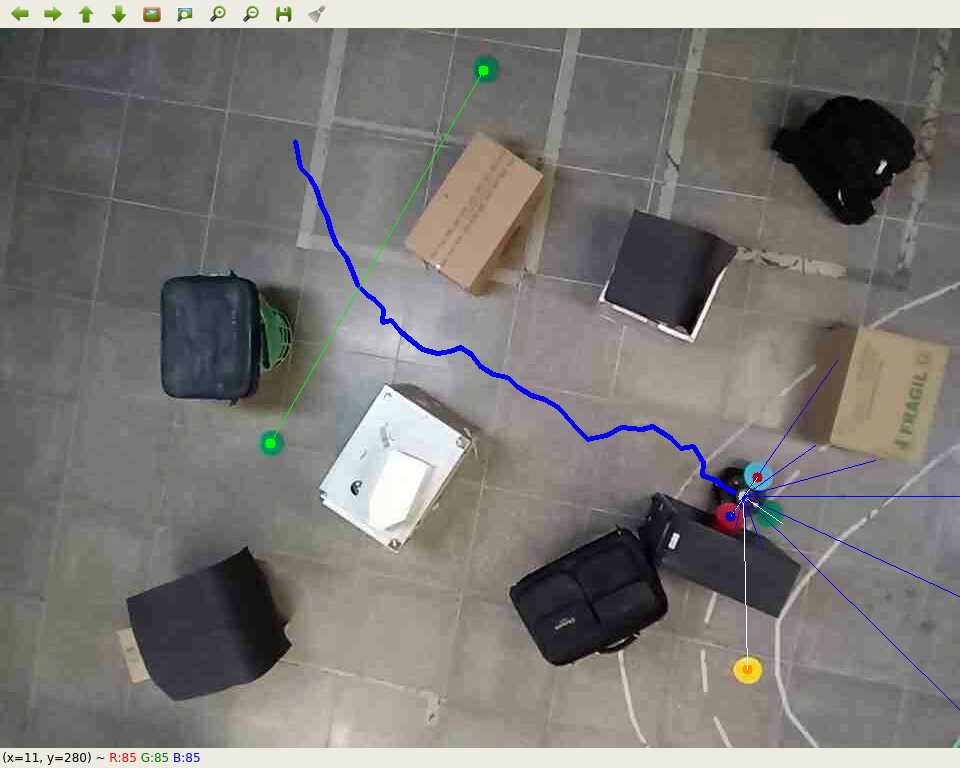
\includegraphics[width=\textwidth]{images/test_env2/6.png}
    \end{subfigure}
    \hfill
    \begin{subfigure}[b]{0.115\textwidth}
        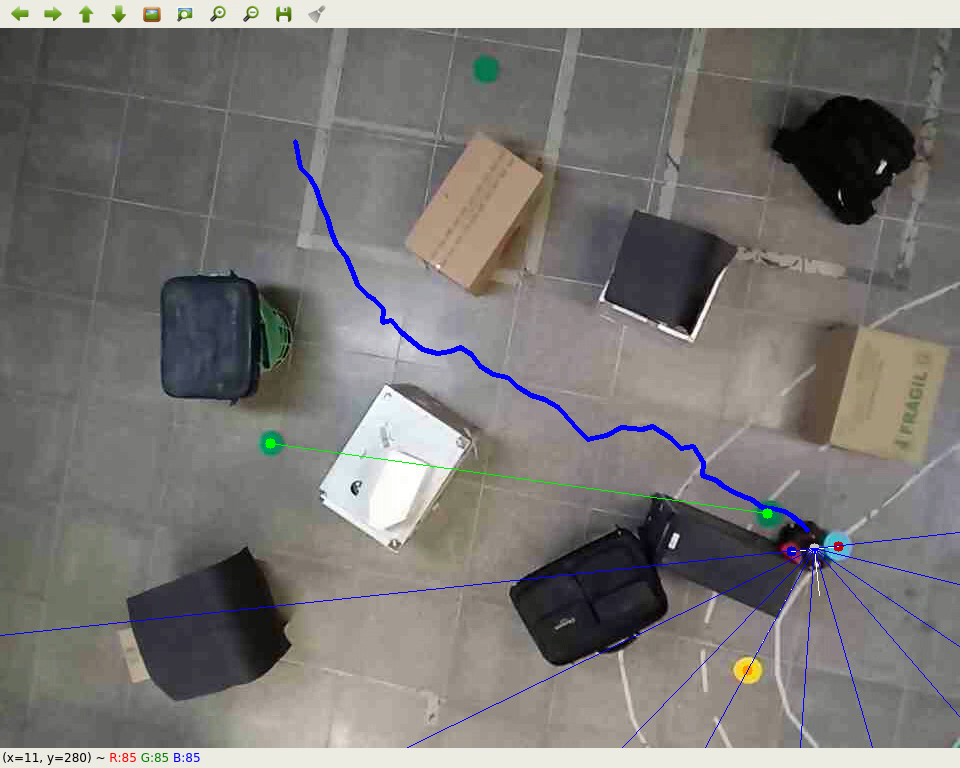
\includegraphics[width=\textwidth]{images/test_env2/7.png}
    \end{subfigure}
    \hfill
    \begin{subfigure}[b]{0.115\textwidth}
        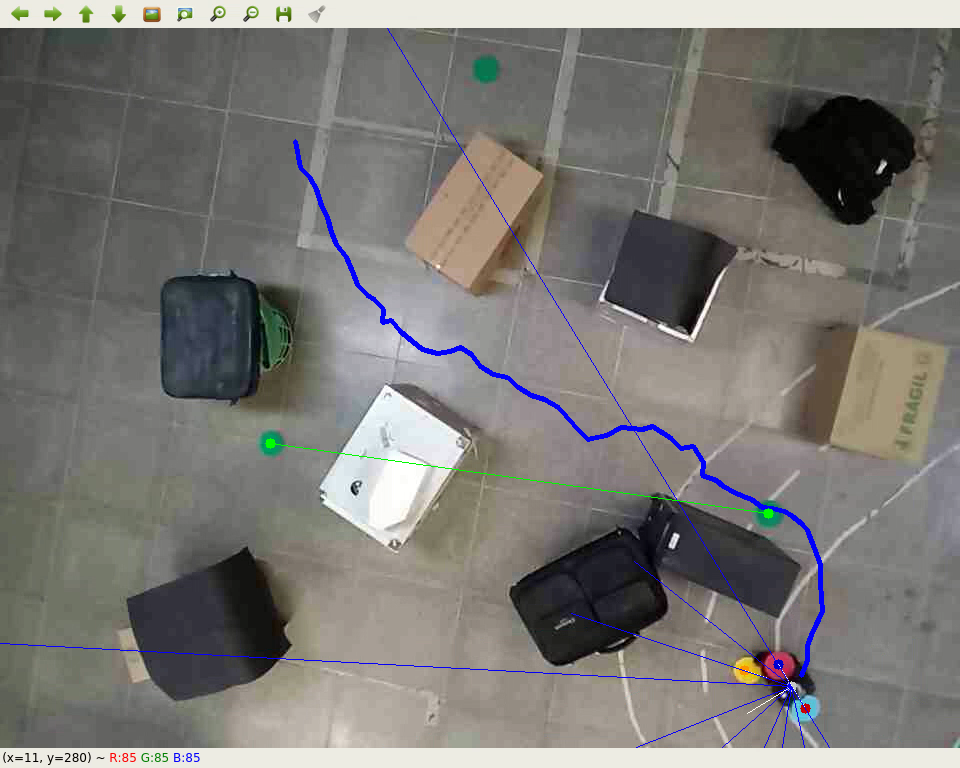
\includegraphics[width=\textwidth]{images/test_env2/8.png}
    \end{subfigure}
    \caption{Images sequence of the experiment on the Turtlebot3 in the second real environment.}\label{fig:frames_env2}
\end{figure}